\documentclass[12pt,]{article}
\usepackage{lmodern}
\usepackage{amssymb,amsmath}
\usepackage{ifxetex,ifluatex}
\usepackage{fixltx2e} % provides \textsubscript
\ifnum 0\ifxetex 1\fi\ifluatex 1\fi=0 % if pdftex
  \usepackage[T1]{fontenc}
  \usepackage[utf8]{inputenc}
\else % if luatex or xelatex
  \ifxetex
    \usepackage{mathspec}
  \else
    \usepackage{fontspec}
  \fi
  \defaultfontfeatures{Ligatures=TeX,Scale=MatchLowercase}
\fi
% use upquote if available, for straight quotes in verbatim environments
\IfFileExists{upquote.sty}{\usepackage{upquote}}{}
% use microtype if available
\IfFileExists{microtype.sty}{%
\usepackage{microtype}
\UseMicrotypeSet[protrusion]{basicmath} % disable protrusion for tt fonts
}{}
\usepackage[margin=1in]{geometry}
\usepackage{hyperref}
\hypersetup{unicode=true,
            pdftitle={Regression models for Cylindrical data in Psychology},
            pdfkeywords={bla vla},
            pdfborder={0 0 0},
            breaklinks=true}
\urlstyle{same}  % don't use monospace font for urls
\usepackage{graphicx,grffile}
\makeatletter
\def\maxwidth{\ifdim\Gin@nat@width>\linewidth\linewidth\else\Gin@nat@width\fi}
\def\maxheight{\ifdim\Gin@nat@height>\textheight\textheight\else\Gin@nat@height\fi}
\makeatother
% Scale images if necessary, so that they will not overflow the page
% margins by default, and it is still possible to overwrite the defaults
% using explicit options in \includegraphics[width, height, ...]{}
\setkeys{Gin}{width=\maxwidth,height=\maxheight,keepaspectratio}
\IfFileExists{parskip.sty}{%
\usepackage{parskip}
}{% else
\setlength{\parindent}{0pt}
\setlength{\parskip}{6pt plus 2pt minus 1pt}
}
\setlength{\emergencystretch}{3em}  % prevent overfull lines
\providecommand{\tightlist}{%
  \setlength{\itemsep}{0pt}\setlength{\parskip}{0pt}}
\setcounter{secnumdepth}{5}
% Redefines (sub)paragraphs to behave more like sections
\ifx\paragraph\undefined\else
\let\oldparagraph\paragraph
\renewcommand{\paragraph}[1]{\oldparagraph{#1}\mbox{}}
\fi
\ifx\subparagraph\undefined\else
\let\oldsubparagraph\subparagraph
\renewcommand{\subparagraph}[1]{\oldsubparagraph{#1}\mbox{}}
\fi

%%% Use protect on footnotes to avoid problems with footnotes in titles
\let\rmarkdownfootnote\footnote%
\def\footnote{\protect\rmarkdownfootnote}

%%% Change title format to be more compact
\usepackage{titling}

% Create subtitle command for use in maketitle
\newcommand{\subtitle}[1]{
  \posttitle{
    \begin{center}\large#1\end{center}
    }
}

\setlength{\droptitle}{-2em}

  \title{Regression models for Cylindrical data in Psychology}
    \pretitle{\vspace{\droptitle}\centering\huge}
  \posttitle{\par}
    \author{}
    \preauthor{}\postauthor{}
    \date{}
    \predate{}\postdate{}
  
\usepackage{booktabs}
\usepackage{longtable}
\usepackage{array}
\usepackage{multirow}
\usepackage[table]{xcolor}
\usepackage{wrapfig}
\usepackage{float}
\usepackage{colortbl}
\usepackage{pdflscape}
\usepackage{tabu}
\usepackage{threeparttable}
\usepackage{threeparttablex}
\usepackage[normalem]{ulem}
\usepackage{makecell}

\usepackage{multirow}
\usepackage{appendix}
\usepackage{color}
\usepackage{hyperref}
\usepackage{subcaption}
\setlength\parindent{24pt}
\usepackage[nodisplayskipstretch]{setspace}\doublespacing
\DeclareRobustCommand{\VANDER}[3]{#2} % set up for citation (in .tex %  place \DeclareRobustCommand{\VANDER}[3]{#3} before bibliography)

\begin{document}
\maketitle
\begin{abstract}
Cylindrical data are multivariate data which consist of a directional,
in this paper circular, and a linear component. Examples of cylindrical
data in psychology include human navigation (direction and distance of
movement), eye-tracking research (direction and length of saccades) and
data from an interpersonal circumplex (type and strength of
interpersonal behavior). In this paper we adapt four models for
cylindrical data to include a regression of the circular and linear
component onto a set of covariates. Subsequently, we illustrate how to
fit these models and interpret their results on a dataset on the
interpersonal behavior of teachers.
\end{abstract}

\section{Introduction}\label{Introduction}

Cylindrical data are data that consist of a linear variable and a
directional variable. In this paper, the directional variable is
circular, meaning that it consists of a single angle instead of a set of
angles. A circular variable is different from a linear variable in the
sense that it is measured on a different scale. Figure \ref{circline}
shows the difference between a circular scale (right) and a linear scale
(left). The most important difference is that on a circular scale the
datapoints 0\(^\circ\) and 360\(^\circ\) are connected and in fact
represent the same number while on a linear scale the two ends,
\(-\infty\) and \(\infty\), are not connected and consequently the
values 0\(^\circ\) and 360\(^\circ\) are located on different places on
the scale. This difference requires us to use special statistical
methods for circular variables (see e.g. Fisher (1995) for an
introduction to circular data and Mardia \& Jupp (2000), Jammalamadaka
\& Sengupta (2001) and Ley \& Verdebout (2017) for a more elaborate
overview). For instance, a notion as simple as the sample average needs
to be re-defined. As is the case for circular data, the analysis of
cylindrical data also requires special methods.\newline
\indent Cylindrical data occur in several fields of research, such as
for instance in meteorology (García-Portugués, Crujeiras, \&
González-Manteiga, 2013), ecology (García-Portugués, Barros, Crujeiras,
González-Manteiga, \& Pereira, 2014) or marine research (Lagona, Picone,
Maruotti, \& Cosoli, 2015). However, also in psychology several types of
cylindrical data can be found. For example, in research on human
navigation in the field of cognitive psychology both the distance, a
linear variable, and the direction, a circular variable, of movement are
of interest (Chrastil \& Warren, 2017). In eye-tracking research,
saccade data are an example of cylindrical data, because both the
direction (\emph{i.e.}, the circular variable) and the duration
(\emph{i.e.}, the linear variable) of the saccades are of interest (for
a review of eye-tracking research see Rayner (2009)).\newline
\indent The type of data that is used in the present study are also
psychological, namely data from circumplex measurement instruments. For
instance, data from the interpersonal circumplex as used in personality
psychology are by definition of a cylindrical nature (see Section
\ref{Example} for a more detailed explanation).\newline
\indent In the literature, several methods have been put forward to
model the relation between the linear and circular component of a
cylindrical variable. Some of these are based on regressing the linear
component onto the circular component using the following type of
relation: \[y = \beta_0 +
\beta_1*\cos(\theta) + \beta_2*\sin(\theta)+ \epsilon,\] where \(y\) is
the linear component and \(\theta\) the circular component (Johnson \&
Wehrly, 1978; Mardia \& Sutton, 1978; Mastrantonio, Maruotti, \&
Jona-Lasinio, 2015). Others model the relation in a different way,
e.g.~by specifying a multivariate model for several linear and circular
variables and modelling their covariance matrix (Mastrantonio, 2018) or
by proposing a joint cylindrical distribution. For example, Abe \& Ley
(2017) introduce a cylindrical distribution based on a Weibull
distribution for the linear component and a sine-skewed von Mises
distribution for the circular component and link these through their
respective shape and concentration parameters. However, none of the
methods that have been proposed thus far include additional covariates
onto which both the circular and linear component are regressed.\newline
\indent Our aim in this paper is to fill this gap in the literature by
adapting four existing cylindrical models in such a way that they
include a regression of both the linear and circular component of a
cylindrical variable onto a set of covariates. From now on we will
therefore refer to the components of the cylindrical variable as outcome
components. Additionally, we will show how a correct statistical
treatment of such cylindrical data can lead to new insights. We will do
this for the teacher data, a dataset from the field of educational
psychology. In the teacher data, apart from modelling the relation
between the linear and circular component of a cylindrical variable we
would also like to predict the two components from a set of covariates
in a regression model.

The paper is organized as follows: Section \ref{Example} describes the
teacher data, while Section \ref{Models} presents the four cylindrical
models and our associated adaptations to new regression models. In that
same section we also discuss the model fit criterion that we will use in
Section \ref{DataAnalysis} for the comparison of the four models. A
detailed data analysis with interesting new insights is also provided in
Section \ref{DataAnalysis}. We conclude the paper with a discussion in
Section \ref{Discussion}, and the Supplementary Material collects the
technical details of the MCMC procedures.

\begin{figure}
\centering
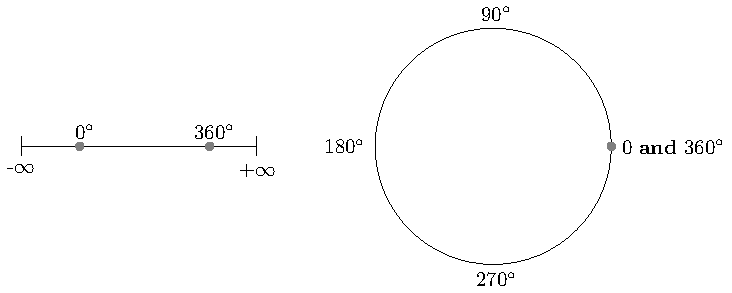
\includegraphics[width = 0.8\textwidth]{Plots/circline.pdf}
\caption{The difference between a linear scale (left) and a circular scale (right).}
\label{circline}
\end{figure}

\section{Teacher data}\label{Example}

\begin{figure}
\centering
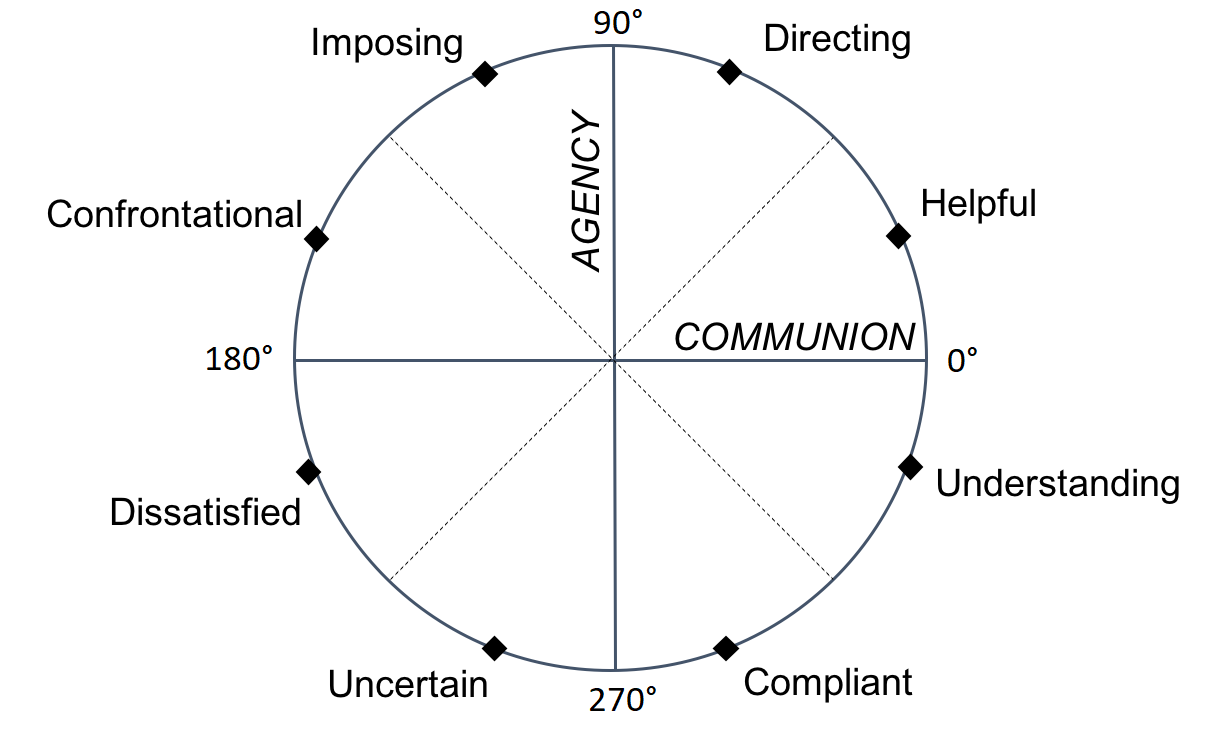
\includegraphics[width = 0.8\textwidth]{Plots/IPC-T.png}
\caption{The interpersonal circle for teachers (IPC-T). The words presented in
the circumference of the circle are anchor words to describe the type of
behavior located in each part of the IPC.}
\label{QTI}
\end{figure}

The motivating example for this article comes from the field of
educational psychology and was collected for the studies on classroom
climate of \VANDER{Want}{Van der}{van der} Want (2015), Claessens (2016)
and Pennings et al. (2018). An indicator of the quality of the classroom
climate is the students' perception of their teachers' interpersonal
behavior. These interpersonal perceptions, both in educational
psychology as well as in other areas of psychology, can be measured
using circumplex measurement instruments (see Horowitz \& Strack (2011)
for an overview of many such instruments).\newline
\indent The circumplex data used in this paper are measured using the
Questionnaire on Teacher Interaction (QTI) (Wubbels, Brekelmans, Brok,
\& Tartwijk, 2006) which is one such circumplex measurement instrument.
The QTI is designed to measure student perceptions of their teachers'
interpersonal behavior and contains items that load on two interpersonal
dimensions: Agency and Communion. Agency refers to the degree of power
or control a teacher exerts in interaction with his/her students.
Communion refers to the degree of friendliness or affiliation a teacher
conveys in interaction with his/her students. The loadings on the two
dimensions of the QTI can be placed in a two-dimensional space formed by
Agency (vertical) and Communion (horizontal), see Figure \ref{QTI}.
Different parts of this space are characterized by different teacher
behavior, e.g. `helpful' or `uncertain'. This two-dimensional space is
called the interpersonal circle/circumplex (IPC). The IPC is ``a
continuous order with no beginning or end'' (Gurtman, 2009, p. 2). We
call such ordering a circumplex ordering and the IPC is therefore often
called the interpersonal circumplex. The ordering also implies that
scores on the IPC could be viewed as a circular variable.\newline
\indent Cremers, Mainhard, \& Klugkist (2018a) explain the circular
nature of the IPC data and analyze them as such using a circular
regression model. The two-dimension scores Agency and Communion can be
converted to a circular score using the two-argument arctangent function
in \eqref{PredVal}, where \(A\) represents a score on the Agency
dimension and \(C\) represents a score on the Communion dimension

\begin{equation}\label{PredVal}
\theta          = \text{atan2}\left(A, \: C\right)  =
\left\{{\begin{array}{lcl}
                                                                       \arctan\left(\frac{A}{C}\right) & \text{if}  \quad&C > 0 \\
\arctan\left(\frac{A}{C}\right) + \pi & \text{if}  \quad& C  <  0  \:\: \&\:\: A \geq 0\\
 \arctan\left(\frac{A}{C}\right) - \pi & \text{if}  \quad&C  <  0 \:\:  \&\:\:A  < 0\\
 +\frac{\pi}{2} & \text{if}  \quad& C  =  0  \:\: \&\:\:A > 0\\
 -\frac{\pi}{2} & \text{if}  \quad& C =  0  \:\: \&\:\:A < 0\\
 \text{undefined} & \text{if} \quad& C =  0   \:\: \&\:\:A = 0.
 \end{array}}
\right.
\end{equation}

The resulting circular variable \(\theta\) can then be modelled and
takes values in the interval \([0, 2\pi)\). However, when
two-dimensional data are converted to the circle we lose some
information, namely the length of the two-dimensional vector
\((A, C)^t\), \emph{i.e.}, its Euclidean norm
\(\mid\mid (A, C)^t \mid\mid\). This length represents the strength of
the type of interpersonal behavior a teacher shows towards his/her
students and can be considered as the linear variable in a cylindrical
model, allowing us to model a circular variable \(\theta\) together with
the linear variable corresponding to \(\mid\mid (A, C)^t \mid\mid\).
This leads to an improved analysis of interpersonal circumplex data as
we take all information into account. In the next section we introduce
several models that can be used for a more accurate and informative
regression analysis on the teacher data. First however we will provide
descriptives for our data set.

\subsection{Data description}\label{DataDescriptives}

The teacher data was collected between 2010 and 2015 and contains
several repeated measures on the IPC of 161 teachers. Measurements were
obtained using the QTI and taken in different years and classes. For
this paper we only consider one measurement, the first occasion (2010)
and largest class if data for multiple classes were available. In
addition to the score on the IPC, the circular outcome, and the strength
of the score on the IPC, the linear outcome, a teachers' self-efficacy
(\verb|SE|) concerning classroom management is used as covariate in the
analysis. After listwise deletion of missings (\(3\) in total, only for
the self-efficacy) we have a sample of 148 teachers. Table
\ref{Tableteacherdescriptives} shows descriptives for the dataset. Here
\(\hat{\rho}\) is a sample estimate for the circular concentration where
a value of 0 means that the data is not concentrated at all, \emph{i.e.}
spread over the entire circle, and a value of 1 means that all data is
concentrated at a single point on the circle. Figure \ref{dataplot} is a
scatterplot showing the relation between the linear and circular outcome
of the teacher data.

\begin{figure}
\centering
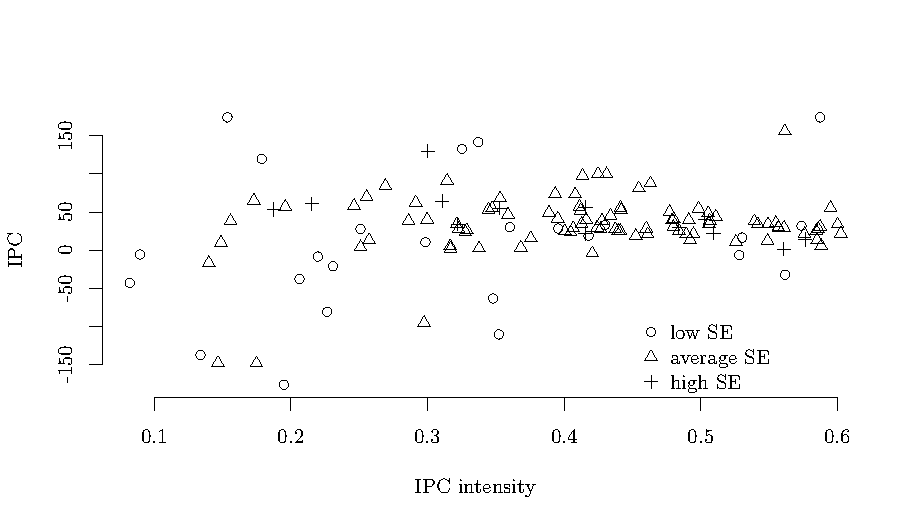
\includegraphics[width = \textwidth]{Plots/dataplot.pdf}
\caption{Plot showing the relation between the linear and circular outcome component (in degrees) of the teacher data.}
\label{dataplot}
\end{figure}

\begin{table}[h]
\centering
\caption{Descriptives for the teacher dataset.} 
\begin{tabular}{lrrrl}
  \noalign{\smallskip}\hline\noalign{\smallskip}
Variable & mean/$\bar{\theta}$ & sd/$\hat{\rho}$ & Range & Type \\ \hline\noalign{\smallskip}
IPC &33.22$^\circ$& 0.76 & - & Circular\\
strength IPC & 0.43 & 0.15 & 0.08 - 0.80 & Linear\\
SE & 5.04 & 1.00 & 1.5 - 7.0 & Linear\\
   \hline
\end{tabular}
\label{Tableteacherdescriptives}
\end{table}

\section{Four cylindrical regression models}\label{Models}

In this section we present four cylindrical models and adapt them such
that they contain predictors for the linear and circular outcomes, \(Y\)
and \(\Theta\). The first two models are based on a construction by
Mastrantonio et al. (2015), while the other models are extensions of the
models from Abe \& Ley (2017) and Mastrantonio (2018).

\subsection{The modified CL-PN and modified CL-GPN  models}\label{CL-(G)PN}

Following Mastrantonio et al. (2015) we consider in this section two
models where the relation between \(\Theta \in [0, 2\pi)\) and
\(Y\in (-\infty, + \infty)\) and \(q\) covariates is specified as

\begin{equation}\label{circlinlink}
Y = \gamma_0 + \gamma_{cos}*\cos(\Theta)*R + \gamma_{sin}*\sin(\Theta)*R + \gamma_1*x_1 + \dots + \gamma_q*x_q +  \epsilon,
\end{equation}

\noindent where the random variable \(R\geq0\) will be introduced below,
the error term \(\epsilon \sim N(0, \sigma^2)\) with variance
\(\sigma^2>0\),
\(\gamma_0, \gamma_{cos}, \gamma_{sin}, \gamma_1, \dots, \gamma_q\) are
the intercept and regression coefficients and \(x_1, \dots, x_q\) are
the \(q\) covariates. In both of these models the conditional
distribution of \(Y\) given \(\Theta=\theta\) and \(R = r\) is given by

\begin{equation}\label{ycondtheta}
f(y \mid \theta, r) = \frac{1}{\sqrt{2\pi\sigma^2}}\exp\left[-\frac{(y - (\gamma_0 + \gamma_1x_1 + \dots + \gamma_qx_q+c))^{2}}{2\sigma^2}\right],\nonumber
\end{equation}

\noindent where
\(c = \begin{bmatrix} r \cos(\theta) \\ r\sin(\theta) \end{bmatrix}^t \begin{bmatrix} \gamma_{cos} \\ \gamma_{sin} \end{bmatrix}\),
\(r \geq 0\). The linear outcome thus has a normal distribution
conditional on \(\Theta\) and \(R\) and contains already linear
covariates \(x_1, \dots, x_q\) in its location part. For the teacher
dataset, the regression equation for the linear outcome in the CL-PN and
CL-GPN model is the following: \[\hat{y}_i =
\gamma_0 + \gamma_{cos}\cos(\theta_i)r_i + \gamma_{sin}\sin(\theta_i)r_i +
\gamma_1\text{SE}_i,\] \noindent where \(\text{SE}_i\) is the
self-efficacy score of one individual \(i = 1, \dots, n\) where \(n\) is
the sample size.\newline
\indent For the circular outcome we assume either a projected normal
(PN) or a general projected normal (GPN) distribution. These
distributions arise from the radial projection of a distribution defined
on the plane onto the circle. The relation between a bivariate vector
\(\boldsymbol{S}\) in the plane and the circular outcome \(\Theta\) is
defined as follows

\begin{equation}\label{projection}
\boldsymbol{S} = \begin{bmatrix} S^{I} \\ S^{II} \end{bmatrix} = R\boldsymbol{u} = \begin{bmatrix} R \cos (\Theta) \\  R\sin (\Theta) \end{bmatrix},
\end{equation}

\noindent where \(R = \mid\mid \boldsymbol{S} \mid\mid\), the Euclidean
norm of the bivariate vector \(\boldsymbol{S}\). In the PN distribution
we assume \(\boldsymbol{S} \sim N_2(\boldsymbol{\mu}, \boldsymbol{I})\)
and in the GPN we assume
\(\boldsymbol{S} \sim N_2(\boldsymbol{\mu}, \boldsymbol{\Sigma})\) where
\(\boldsymbol{\mu} \in \mathbb{R}^2\),
\(\boldsymbol{\Sigma} = \begin{bmatrix} \tau^2 + \rho^2 & \rho\\ \rho & 1 \end{bmatrix}\),
\(\rho \in (-\infty, +\infty)\) and \(\tau^2 \geq 0\) (as in
Hernandez-Stumpfhauser, Breidt, \& Woerd (2016)). This leads to the
circular-linear PN (CL-PN) and circular-linear GPN (CL-GPN)
distributions. We will now detail how we modify both cylindrical
distributions to also incorporate covariates for the circular part.

\subsubsection{The modified CL-PN distribution}

Following Nuñez-Antonio, Gutiérrez-Peña, \& Escarela (2011), the joint
density of \(\Theta\) and \(R\) for the PN distribution equals

\begin{equation}\label{pnreg}
f(\theta,r \mid \boldsymbol{\mu}, \boldsymbol{I}) = \frac{r}{2\pi} \exp\left[- \frac{(r\boldsymbol{u} - \boldsymbol{\mu})^t(r\boldsymbol{u} - \boldsymbol{\mu})}{2}\right],
\end{equation}

\noindent where
\(\boldsymbol{u}= \begin{bmatrix} \cos (\theta) \\ \sin (\theta) \end{bmatrix}\)
and \(r\) is the same as in \eqref{circlinlink} and \eqref{ycondtheta}
and is defined in \eqref{projection}. In a regression setup the outcomes
\(\theta_i,r_i\) for each individual \(i = 1, \dots, n\), where \(n\) is
the sample size, are generated independently from the distribution with
density \eqref{pnreg}. The mean vector
\(\boldsymbol{\mu}_i \in \mathbb{R}^2\) is then defined as
\(\boldsymbol{\mu}_i = \boldsymbol{B}^t\boldsymbol{z}_i\) where the
vector \(\boldsymbol{z}_i\) is a vector of dimension \(p + 1\) that
contains the covariate values and the value 1 to estimate an intercept
and
\(\boldsymbol{B} = (\boldsymbol{\beta}^{I}, \boldsymbol{\beta}^{II})\)
contains the regression coefficients and intercepts. Note however that
the dimensions of \(\boldsymbol{\beta}^{I}\) and
\(\boldsymbol{\beta }^{II}\) need not necessarily be the same and we are
thus allowed to have a different set of predictor variables and vectors
\(\boldsymbol{z}_i^I\) and \(\boldsymbol{z}_i^{II}\) for the two
components of \(\boldsymbol{\mu}_i\). For the teacher dataset, the
regression equation for the circular outcome in the CL-PN model is
\[\hat{\boldsymbol{\mu}}_{i} = \begin{pmatrix} \mu_{i}^{I}  \\ \mu_{i}^{II}
\end{pmatrix}=\begin{pmatrix} \beta_0^{I} + \beta_1^{I}\text{SE}_i  \\
\beta_0^{II} + \beta_1^{II}\text{SE}_i \end{pmatrix}.\]

\subsubsection{The modified CL-GPN distribution}

Following Wang \& Gelfand (2013) and Hernandez-Stumpfhauser et al.
(2016) the joint density of \(R\) and \(\Theta\) for the GPN
distribution equals

\begin{equation}\label{gpnreg}
f(\theta, r \mid \boldsymbol{\mu}, \boldsymbol{\Sigma}) = \frac{r}{2\pi\tau} \exp\left[ -\frac{(r\boldsymbol{u}-\boldsymbol{\mu})^{t}\boldsymbol{\Sigma}^{-1}(r\boldsymbol{u}-\boldsymbol{\mu})}{2}\right],
\end{equation}

\noindent where we recall that
\(\boldsymbol{\Sigma} = \begin{bmatrix} \tau^2 + \rho^2 & \rho\\ \rho & 1 \end{bmatrix}\).
In a regression setup the outcomes \(\theta_i\) and \(r_i\) for each
individual are generated independently from \eqref{gpnreg}. The mean
vector \(\boldsymbol{\mu}_i \in \mathbb{R}^2\) is defined in the same
way via covariates as for the modified CL-PN distribution. Note in
contrast with the CL-PN model where \(\boldsymbol{z}_i^I\) and
\(\boldsymbol{z}_i^{II}\) are allowed to differ we do need to have the
same predictors for both components of \(\boldsymbol{\mu}_i\) in the
CL-GPN model. This is due to the fact that the variance-covariance
matrix \(\boldsymbol{\Sigma}\) is no longer identity. For the teacher
dataset, the regression equation for the circular outcome in the CL-GPN
model is the same as in the CL-PN model.

\subsubsection{Parameter estimation}

Both cylindrical models introduced here are estimated using Markov Chain
Monte Carlo (MCMC) methods based on Nuñez-Antonio et al. (2011), Wang \&
Gelfand (2013) and Hernandez-Stumpfhauser et al. (2016) for the
regression of the circular outcome. A detailed description of the
Bayesian estimation and MCMC samplers can be found in the Supplementary
Material.

\subsection{The modified Abe-Ley model}\label{WeiSSVM}

This model is an extension of the cylindrical model introduced in Abe \&
Ley (2017) to the regression context. The joint density of \(\Theta\)
and \(Y\), in this model defined only on the positive real half-line
\([0, + \infty)\), reads

\begin{equation}\label{WeiSSVMdensity}
f(\theta, y) = \frac{\alpha\beta^\alpha}{2\pi\cosh(\kappa)}
                 (1 +\lambda\sin(\theta - \mu))
                 y^{\alpha-1}
                 \exp[-(\beta y)^{\alpha}(1-\tanh(\kappa)\cos(\theta - \mu))],
\end{equation}

\noindent where \(\alpha > 0\) is a linear shape parameter,
\(\kappa > 0\) and \(\lambda \in [-1, 1]\) are circular concentration
and skewness parameters with \(\kappa\) also regulating the
circular-linear dependence. Our modification occurs at the level of the
linear scale parameter \(\beta>0\) and circular location parameter
\(\mu\in [0, 2\pi)\), both of which we express in terms of covariates:
\(\beta_i = \exp(\boldsymbol{x}_i^t\boldsymbol{\nu}) > 0\) and
\(\mu_i = \eta_0 + 2\tan^{-1}(\boldsymbol{z}_i^t\boldsymbol{\eta})\).
The parameter \(\boldsymbol{\nu}\) is a vector of \(q\) regression
coefficients \(\nu_j \in (-\infty, +\infty)\) for the prediction of
\(y\) where \(j = 0, \dots, q\) and \(\nu_0\) is the intercept. The
parameter \(\eta_0 \in [0, 2\pi)\) is the intercept and
\(\boldsymbol{\eta}\) is a vector of \(p\) regression coefficients
\(\eta_j \in (-\infty, +\infty)\) for the prediction of \(\theta\) where
\(j = 1, \dots, p\). The vector \(\boldsymbol{x}_i\) is a vector of
predictor values for the prediction of \(y\) and \(\boldsymbol{z}_i\) is
a vector of predictor values for the prediction of \(\theta\). In a
regression setup the outcome vector \((\theta_i, y_i)^t\) for each
individual is generated independently from the modified density
\eqref{WeiSSVMdensity}.\newline
\indent As in Abe \& Ley (2017), the conditional distribution of \(Y\)
given \(\Theta=\theta\) is a Weibull distribution with shape \(\alpha\)
and scale \(\beta(1-\tanh(\kappa)\cos(\theta - \mu))^{1/\alpha}\) and
the conditional distribution of \(\Theta\) given \(Y=y\) is a sine
skewed von Mises distribution with location parameter \(\mu\) and
concentration parameter \((\beta y)^\alpha\tanh(\kappa)\). The
log-likelihood for this model equals

\begin{align}\label{WeiSSVMLikelihood}
l(\alpha, \boldsymbol{\nu}, \lambda, \kappa, \boldsymbol{\eta}) 
   &= n[\ln(\alpha) - \ln(2\pi\cosh(\kappa))] + \alpha \sum^{n}_{i = 1} \boldsymbol{x}_i^t\boldsymbol{\nu} \nonumber\\
   &\:\:\:\:+\sum^{n}_{i = 1} \ln(1 +\lambda\sin(\theta_i - \eta_0 - 2\tan^{-1}(\boldsymbol{z}_i^t\boldsymbol{\eta}))) 
   +(\alpha-1)\sum^{n}_{i = 1} \ln(y_i) \nonumber\\
   &\:\:\:\:-\sum^{n}_{i = 1}( \exp(\boldsymbol{x}_i^t\boldsymbol{\nu})y_i)^{\alpha}(1-\tanh(\kappa)\cos(\theta_i - \eta_0 - 2\tan^{-1}(\boldsymbol{z}_i^t\boldsymbol{\eta}))).\nonumber
\end{align}

\noindent For the teacher data, \(\boldsymbol{z} = \boldsymbol{x}\) and
the regression equations for the circular and linear outcomes in the
Abe-Ley model are: \[\hat{\mu}_{i} = \eta_0 + 2 *
\tan^{-1}(\eta_1\text{SE}_i),\] and \[\hat{\beta}_{i} = \exp(\nu_0 +
\nu_1\text{SE}_i).\] \noindent We can use numerical optimization
(Nelder-Mead) to find solutions for the maximum likelihood (ML)
estimates for the parameters of the model.

\subsection{Modified joint projected and skew normal (GPN-SSN)}\label{CL-GPN_multivariate}

This model is an extension of the cylindrical model introduced by
Mastrantonio (2018) to the regression context. Both models contain \(m\)
independent circular outcomes and \(w\) independent linear outcomes. The
circular outcomes
\(\boldsymbol{\Theta} = (\boldsymbol{\Theta}_1, \dots,  \boldsymbol{\Theta}_m)\)
are modelled together by a multivariate GPN distribution. The joint
distribution of \(\boldsymbol{\Theta}\) and \(\boldsymbol{R}\) can thus
be modeled as the product of (\ref{gpnreg}) for each of the \(m\)
circular outcomes. The linear outcomes
\(\boldsymbol{Y} = (\boldsymbol{Y}_1,  \dots, \boldsymbol{Y}_w)\) are
modelled together by a multivariate skew normal distribution (Sahu, Dey,
\& Branco, 2003). Because the GPN distribution is modelled using a
so-called augmented representation (as in \eqref{projection} and
\eqref{gpnreg}) it is convenient to use a similar tactic for modelling
the multivariate skew normal distribution. Following Mastrantonio (2018)
the linear outcomes are represented as
\[\boldsymbol{Y} = \boldsymbol{\mu}_y + \boldsymbol{\Lambda}\boldsymbol{D} + \boldsymbol{H},\]
\noindent where \(\boldsymbol{\mu}_y\) is a mean vector for the linear
outcome \(\boldsymbol{Y}\),
\(\boldsymbol{\Lambda} = \text{diag}(\boldsymbol{\lambda})\) is a
\(w \times w\) diagonal matrix with diagonal elements
\(\lambda_1, \dots, \lambda_w\) (skewness parameters),
\(\boldsymbol{D} \sim HN_w(\boldsymbol{0}_w, \boldsymbol{I}_w)\), a
\(w\)-dimensional half normal distribution (Olmos, Varela, Gómez, \&
Bolfarine, 2012), and
\(\boldsymbol{H} \sim N_w(\boldsymbol{0}_w, \boldsymbol{\Sigma}_y)\).
This means that, conditional on the auxiliary data \(\boldsymbol{D}\),
\(\boldsymbol{Y}\) is normally distributed with mean
\(\boldsymbol{\mu}_y + \boldsymbol{\Lambda}\boldsymbol{D}\) and
covariance matrix \(\boldsymbol{\Sigma}_y\). The joint density for
\((\boldsymbol{Y}^t, \boldsymbol{D}^t)^t\) is defined as:

\begin{equation}\label{YDjoint}
f(\boldsymbol{y}, \boldsymbol{d}) = 2^w\phi_w(\boldsymbol{y} \mid \boldsymbol{\mu}_y + \boldsymbol{\Lambda}\boldsymbol{d}, \boldsymbol{\Sigma}_y) \phi_w(\boldsymbol{d} \mid \boldsymbol{0}_w, \boldsymbol{I}_w),\nonumber
\end{equation}

\noindent where
\(\phi_\ell(\cdot|\boldsymbol{\mu}_\ell,\boldsymbol{\Sigma}_\ell)\)
stands for the \(\ell\)-dimensional normal density with mean vector
\(\boldsymbol{\mu}_\ell\) and covariance \(\boldsymbol{\Sigma}_\ell\).
As in Mastrantonio (2018) dependence between the linear and circular
outcome is created by modelling the augmented representations of
\(\boldsymbol{\Theta}\) and \(\boldsymbol{Y}\) together in a \(2m + w\)
dimensional normal distribution. The joint density of the model is then
represented by:

\begin{equation}\label{YDThetarjoint} 
f(\boldsymbol{\theta}, \boldsymbol{r},
\boldsymbol{y}, \boldsymbol{d}) = 2^w\phi_{2m+w}((\boldsymbol{s}^t,
\boldsymbol{y}^t)^t \mid \boldsymbol{\mu} + (\boldsymbol{0}_{2m}^t, ({\rm
diag}(\boldsymbol{\lambda})\boldsymbol{d})^t)^t, \boldsymbol{\Sigma})
\phi_w(\boldsymbol{d} \mid \boldsymbol{0}_w, \boldsymbol{I}_w) \prod_{j =
1}^{m}r_j, 
\end{equation}

\noindent where
\(\boldsymbol{s} = (r_1(\cos(\theta_1), \sin(\theta_1)), \dots, r_m(\cos(\theta_m), \sin(\theta_m)))^t\),
the mean vector
\(\boldsymbol{\mu} = (\boldsymbol{\mu}_s^t, \boldsymbol{\mu}_y^t)^t\)
and
\(\boldsymbol{\Sigma} = \left ( \begin{matrix} \boldsymbol{\Sigma}_s & \boldsymbol{\Sigma}_{sy} \\ \boldsymbol{\Sigma}_{sy}^t & \boldsymbol{\Sigma}_y \\ \end{matrix} \right )\).
The matrix \(\boldsymbol{\Sigma}_s\) is the covariance matrix for the
variances of and covariances between the augmented representations of
the circular outcome and the matrix \(\boldsymbol{\Sigma}_{sy}\)
contains covariances between the augmented representations of the
circular outcome and the linear outcome. \newline
\indent In our regression extension we have \(i = 1, \dots, n\)
observations of \(m\) circular outcomes, \(w\) linear outcomes and \(g\)
covariates. The mean in the density in \eqref{YDThetarjoint} then
becomes \(\boldsymbol{\mu}_i = \boldsymbol{B}^t\boldsymbol{x}_i\) where
\(\boldsymbol{B}\) is a \((g + 1) \times (2m + w)\) matrix with
regression coefficients and intercepts and \(\boldsymbol{x}_i\) is a
\(g + 1\) dimensional vector containing the value 1 to estimate an
intercept and the \(g\) covariate values. \newline
\indent For the teacher data, the regression equations for the circular
and linear outcomes in the GPN-SSN model are
\[\hat{\boldsymbol{\mu}}_{i} = \boldsymbol{\beta}_0 +
\boldsymbol{\beta}_1\text{SE}_i,\] where
\(\hat{\boldsymbol{\mu}}_i = (\hat{\boldsymbol{\mu}}_{s_i}^t, \hat{\mu}_{y_i})^t\),
\(\boldsymbol{\beta}_0 = (\beta_{0_{s^{I}}}, \beta_{0_{s^{II}}},\beta_{0_y})^t\)
and
\(\boldsymbol{\beta}_1 = (\beta_{1_{s^{I}}}, \beta_{1_{s^{II}}},\beta_{1_y})^t\).
Note that because \(m = 1\) and \(w = 1\), \(\boldsymbol{\mu}_{s_i}\) is
a 2 dimensional vector and \(\mu_{y_i}\) is a scalar. We estimate the
model using MCMC methods. A detailed description of these methods is
given in the Supplementary Material.

\subsection{Model fit criterion}\label{Modelfit}

For the four cylindrical models we focus on their out-of-sample
predictive performance to determine the fit of the model. To do so we
use k-fold cross-validation and split our data into 10 folds. Each of
these folds (10 \(\%\) of the sample) is used once as a holdout set and
9 times as part of a training set. The analysis will thus be performed
10 times, each time on a different training set.\newline
\indent A proper criterion to compare out-of-sample predictive
performance is the Predictive Log Scoring Loss (PLSL) (Gneiting \&
Raftery, 2007). The lower the value of this criterion, the better the
predictive performance of the model. Using ML estimates this criterion
can be computed as follows:

\begin{equation}\label{PLSLML}
PLSL = -2 \sum_{i = 1}^{M}\log l(x_i \mid \hat{\boldsymbol{\vartheta}}),\nonumber
\end{equation}

\noindent where \(l\) is the model likelihood, \(M\) is the sample size
of the holdout set, \(x_i\) is the \(i^{th}\) datapoint from the holdout
set and \(\hat{\boldsymbol{\vartheta}}\) are the ML estimates of the
model parameters. Using posterior samples the criterion is similar to
the log pointwise predictive density (lppd) (Gelman et al., 2014, p.
169) and can be computed as:

\begin{equation}\label{PLSLBayes}
PLSL = -2 \frac{1}{B} \sum_{j = 1}^{B}\sum_{i = 1}^{M} \log l(x_i \mid \boldsymbol{\vartheta}^{(j)}),\nonumber
\end{equation}

\noindent where \(B\) is the amount of posterior samples and
\(\boldsymbol{\vartheta}^{(j)}\) are the posterior estimates of the
model parameters for the \(j^{th}\) iteration. Because the joint density
and thus also the likelihood for the modified GPN-SSN model in
(\ref{YDThetarjoint}) is not available in closed form (Mastrantonio,
2018) we compute the PLSL for the circular and linear outcome separately
for all models. Note that although we fit the CL-PN, CL-GPN and GPN-SSN
models using Bayesian statistics, we do not take prior information into
account when assessing model fit with the PLSL. According to Gelman et
al. (2014) this is not necessary since we are assessing the fit of a
model to data, the holdout set, only. They argue that the prior in such
case is only of interest for estimating the parameters of the model but
not for determining the predictive accuracy.\newline
\indent We use the loglikelihoods of the following conditional densities
for the computation of the PLSL in the teacher data:

\begin{itemize}
\item For the modified CL-PN model:

$y_i \mid \mu_i, \sigma^2 \sim N(\mu_i, \sigma^2)$, where $\mu_i = \hat{y}_i$ and for $\theta_i$ we use \eqref{pnreg}.

\item For the modified CL-GPN model:

$y_i \mid \mu_i, \sigma^2 \sim N(\mu_i, \sigma^2)$, where $\mu_i = \hat{y}_i$ and for $\theta_i$ we use \eqref{gpnreg}.

\item For the modified Abe-Ley model:

$y_i \mid \theta_i, \beta_i, \mu_i, \kappa, \alpha \sim W\left(\beta_i(1-\tanh(\kappa)\cos(\theta_i - \mu_i))^{1/\alpha}, \alpha\right)$, a Weibull distribution.

$\theta_i \mid y_i, \beta_i, \mu_i, \kappa, \alpha, \lambda \sim SSVM\left(\mu_i, (\beta_iy_i)^{\alpha}(\tanh{\kappa})\right)$, a sine-skewed von Mises distribution.

\item For the modified joint projected and skew normal model:

$y_i \mid \boldsymbol{\mu}_i, \boldsymbol{\Sigma}, \theta_i, r_i \sim SSN(\mu_{i_y} + \lambda d_i + \boldsymbol{\Sigma}_{sy}^t\boldsymbol{\Sigma}_s^{-1}(\boldsymbol{s}_i - \boldsymbol{\mu}_{i_s}), \sigma^2_y + \boldsymbol{\Sigma}_{sy}^t\boldsymbol{\Sigma}_s^{-1}\boldsymbol{\Sigma}_{sy}),$

$\theta_i \mid \boldsymbol{\mu}_i, \boldsymbol{\Sigma}, y_i, d_i \sim GPN(\boldsymbol{\mu}_{i_s} + \boldsymbol{\Sigma}_{sy}\sigma^{-2}_y(y_i - \mu_{i_y} - \lambda d_i), \boldsymbol{\Sigma}_s + \boldsymbol{\Sigma}_{sy}\sigma_y^{-2}\boldsymbol{\Sigma}_{sy}^t)$

where $SSN$ is the skew normal distribution.
\end{itemize}

\noindent For each of the four cylindrical models and for each of the 10
cross-validation analyses we can then compute a PLSL for the circular
and linear outcome by using the conditional log-likelihoods of the
respective outcome. To evaluate the predictive performance we average
across the PLSL criteria of the cross-validation analyses. We also
assess the cross-validation variability by means of the standard
deviations of the PLSL criteria.

\section{Data Analysis}\label{DataAnalysis}

In this section we analyze the teacher data with the help of the four
cylindrical models from Section \ref{Models}. We will present the
results, posterior estimates and their interpretation, per model and
finish with a section comparing the fit of the different models.

\subsection{Results \& Analysis}\label{DataResults}

In the Supplementary Material we have described the starting values for
the MCMC procedures, hence it remains to specify the starting values for
the maximum likelihood based Abe-Ley model:
\(\eta_0 = 0.9, \eta_1 = 0.9, \nu_0 = 0.9, \nu_1 = 0.9, \kappa = 0.9, \alpha = 0.9, \lambda = 0\).
The initial amount of iterations for the three MCMC samplers was set to
2000. After convergence checks via traceplots we concluded that some of
the parameters of the GPN-SSN model did not converge. Therefore we set
the amount of iterations of the MCMC models to 20,000 and subtracted a
burn-in of 5000 to reach convergence. Note that we choose the same
amount of iterations for all three Bayesian models to make their
comparison via the PLSL as fair as possible. Lastly, the predictor
\verb|SE| was centered before inclusion in the analysis as this allows
the intercepts to bear the classical meaning of average behavior.

\subsubsection{The modified CL-PN and CL-GPN models} \label{resCL(G)PN}

\begin{table}

\caption{\label{tab:estCLGPN}Results, cross-validation mean and standard deviation, for the modified CL-PN and CL-GPN models}
\centering
\begin{tabular}[t]{lllllll}
\toprule
\multicolumn{1}{c}{Parameter} & \multicolumn{3}{c}{CL-PN} & \multicolumn{3}{c}{CL-GPN} \\
\cmidrule(l{2pt}r{2pt}){1-1} \cmidrule(l{2pt}r{2pt}){2-4} \cmidrule(l{2pt}r{2pt}){5-7}
  & Mode & HPD LB & HPD UB & Mode & HPD LB & HPD UB\\
\midrule
$\beta_0^{I}$ & 1.76 (0.09) & 1.50 (0.07) & 0.09 (0.09) & 2.42 (0.15) & 1.90 (0.10) & 3.05 (0.17)\\
$\beta_1^{I}$ & 0.65 (0.07) & 0.42 (0.06) & 0.08 (0.08) & 0.85 (0.12) & 0.45 (0.09) & 1.30 (0.15)\\
$\beta_0^{II}$ & 1.15 (0.05) & 0.92 (0.04) & 0.04 (0.04) & 1.47 (0.05) & 1.17 (0.04) & 1.79 (0.05)\\
$\beta_1^{II}$ & 0.58 (0.03) & 0.38 (0.04) & 0.04 (0.04) & 0.70 (0.08) & 0.46 (0.05) & 0.96 (0.07)\\
$\gamma_0$ & 0.38 (0.01) & 0.31 (0.01) & 0.01 (0.01) & 0.37 (0.01) & 0.31 (0.01) & 0.42 (0.01)\\
\addlinespace
$\gamma_{cos}$ & 0.04 (0.00) & 0.01 (0.00) & 0.00 (0.00) & 0.03 (0.00) & 0.01 (0.00) & 0.05 (0.00)\\
$\gamma_{sin}$ & -0.01 (0.00) & -0.04 (0.00) & 0.00 (0.00) & -0.00 (0.00) & -0.03 (0.00) & 0.03 (0.00)\\
$\gamma_1$ & 0.03 (0.01) & -0.00 (0.00) & 0.07 (0.01) & 0.03 (0.01) & -0.00 (0.00) & 0.06 (0.00)\\
$\sigma$ & 0.14 (0.00) & 0.12 (0.00) & 0.00 (0.00) & 0.14 (0.00) & 0.12 (0.00) & 0.16 (0.00)\\
$\sum_{1,1}$ & NA (NA) & NA (NA) & NA (NA) & 3.02 (0.25) & 1.83 (0.14) & 5.02 (0.41)\\
\addlinespace
$\sum_{1,2}$ & NA (NA) & NA (NA) & NA (NA) & 0.46 (0.12) & 0.12 (0.12) & 0.80 (0.10)\\
$\sum_{2,2}$ & NA (NA) & NA (NA) & NA (NA) & 1.00 (0.00) & 1.00 (0.00) & 1.00 (0.00)\\
\bottomrule
\end{tabular}
\end{table}

\begin{table}
\caption{\label{tab:means}Posterior estimates (in degrees) for the circular mean in the CL-PN, CL-GPN and GPN-SSN models}
\centering
\begin{tabular}[t]{lrrr}
\toprule
  & Mode & HPD LB & HPD UB\\
  \midrule
Cl-PN & 32.29 & 24.81 & 39.71\\
CL-GPN & 33.70 & 26.72 & 41.15\\
GPN-SSN & 35.30 & 28.31 & 43.10\\
\bottomrule
\multicolumn{4}{l}{\textsuperscript{a} Note that these means are based on}\\
\multicolumn{4}{l}{the posterior predictive}\\
\multicolumn{4}{l}{distribution for the intercepts}\\
\multicolumn{4}{l}{following (Wang \& Gelfand, 2013).}\\
\end{tabular}
\end{table}

First recall the regression equations predicting the linear outcome
\[\hat{y}_i = \gamma_0 + \gamma_{cos}\cos(\theta_i)r_i + \gamma_{sin}\sin(\theta_i)r_i + \gamma_1\text{SE}_i\]
\noindent and circular outcome
\[\hat{\boldsymbol{\mu}}_{i} = \begin{pmatrix}
  \mu_{i}^{I}  \\
\mu_{i}^{II}
 \end{pmatrix}=\begin{pmatrix}
  \beta_0^{I} + \beta_1^{I}\text{SE}_i  \\
  \beta_0^{II} + \beta_1^{II}\text{SE}_i
 \end{pmatrix}.\] \noindent  For both models, \(\hat{y}\) is the
predicted strength of interpersonal behavior, \(\hat{\boldsymbol{\mu}}\)
is the predicted mean vector of the type of interpersonal behavior and
the \(\gamma\)'s and \(\beta\)'s are intercepts and regression
coefficients.\newline \indent Table \ref{tab:estCLGPN} shows the results
for the modified CL-PN and CL-GPN models fit to the teacher dataset. The
estimates in this table are the averages and standard deviations of the
10 cross-validation estimates. We show both the estimated posterior mode
and the 95\% highest posterior density (HPD) interval for each
parameter. The posterior estimates for the \(\beta\)'s and \(\gamma\)'s
are quite similar for both models. We also see this similarity when we
look at the predicted circular and linear means. The predicted linear
mean is equal to \(\gamma_0\) which is equal to 0.38 and 0.37 in the
CL-PN and CL-GPN models, respectively. The predicted circular means can
be computed from \(\beta_0^{I}\) and \(\beta_0^{II}\) using a double
arctangent function \(\mbox{atan2}(\beta_0^{II}, \beta_0^{I})\), see
\eqref{PredVal}. If we do this at each iteration of the MCMC sampler we
get the posterior distribution of the circular mean in both models.
Table \ref{tab:means} shows the posterior mode of the estimated circular
means, which are very similar (32.29\(^\circ\) and
33.54\(^\circ\)).\newline
\indent Next we investigate the effect of self-efficacy. In the CL-PN
model we can transform the regression parameters on the two components
\(I\) and \(II\) to one circular regression coefficient \(b_c\) using
the methods described by Cremers, Mulder, \& Klugkist (2018b). The
dashed line in Figure \ref{regline} shows the predicted regression line
from the CL-PN model. Here \(b_c\) is the slope of this line at the
inflection point (black square) and its posterior mode is estimated at
1.67 (-24.66,
29.33)\footnote{Note that this is a linear approximation to the
circular regression line representing the slope at a specific point. Therefore
it is possible for the HPD interval to be wider than $2\pi$. In this case the
interval is much wider and covers 0, indicating there is no evidence to reject
the null-hypothesis of no effect.}. Even though the HPD of \(b_c\)
includes 0, indicating there is no evidence to reject the null-hypotheis
of no effect, we continue with its interpretation for eductional
purposes. The interpretation of \(b_c\) is that at the inflection point
an increase of 1 unit in self-efficacy leads to an increase of
\(1.67*(180/\pi) = 95.68^\circ\) in the type of interpersonal
behavior..However, as we can see in Figure \ref{regline} the inflection
point lies almost outside the range of the actual data. Instead of
looking at the inflection point we might compute the slope of the
regression line at the average self-efficacy. This parameter we call the
slope at the mean (\(SAM\)) (Cremers et al., 2018b) and it is estimated
at 0.02 (0.01; 0.04) for our data. This means that at the average
self-efficacy an increase of 1 unit only leads to an increase of
\(0.02*(180/\pi) = 1.15^\circ\) in the type of interpersonal behavior.
The HPD of the \(SAM\) does not include 0 which means that the effect at
the average self-efficacy can be distinguished from 0.\newline
\indent In the CL-GPN model we cannot compute circular regression
coefficients such as the \(b_c\) and \(SAM\) computed above due to the
fact that not only the mean vector \(\boldsymbol{\mu}\) but also the
covariance matrix \(\boldsymbol{\Sigma}\) influences the predicted value
on the circle. Instead, we will compute posterior predictive
distributions for the predicted circular outcome of individuals scoring
the minimum, maximum and median self-efficacy. The modes and 95\% HPD
intervals of these posterior predictive distributions are
\(\hat{\theta}_{SE_{min}} = 215.74^\circ (147.36^\circ, \: 44.49^\circ)\),
\(\hat{\theta}_{SE_{median}} = 25.93^\circ (337.02^\circ, \: 138.59^\circ)\),
\(\hat{\theta}_{SE_{max}} = 30.86^\circ (8.63^\circ, \: 72.19^\circ)\).
Note that we display the modes and HPD intervals for the posterior
predictive distributions on the interval \([0^\circ, 360^\circ)\). Note
that \(44.49^\circ = 404.49^\circ\) due to the periodicity of a circular
variable. The posterior mode estimate of \(215.74^\circ\) thus lies
within its HPD interval \((147.36^\circ, \: 44.49^\circ)\).The HPD
intervals of the three posterior predictive distributions overlap. Had
they not overlapped we could have concluded that as the self-efficacy
increases, the score of the teacher on the IPC moves counterclockwise.
\newline
\indent The effect of self-efficacy on the strength of interpersonal
behavior is quantified by \(\gamma_1\) in both the CL-PN and CL-GPN
models. This parameter can be interpreted in the same way as in a usual
regression model. The HPD interval of \(\gamma_1\) includes 0 which
means that there is not enough evidence for an effect of self-efficacy
on the strength of interpersonal behavior. Note that the lower bounds of
the HPD interval of this parameter are however very close to
zero.\newline
\indent  The relation between the circular and linear outcome, that is,
between type of interpersonal behavior and strength of interpersonal
behavior, is described by the parameters \(\gamma_{\cos}\) and
\(\gamma_{\sin}\). The HPD interval of \(\gamma_{\cos}\) does not
include 0 for both the CL-PN and CL-GPN models, meaning that the cosine
component of the type of interpersonal behavior has an effect on the
strength of interpersonal behavior. In the teacher data the sine and
cosine components have a substantive meaning. In this case the Communion
(cosine) component of the IPC positively effects the strength of a
teachers' type of interpersonal behavior, in plain words: teachers
exhibiting interpersonal behavior types with higher communion scores
(e.g., `helpful' and `understanding' in Figure 2) are stronger in their
behavior.

\begin{figure}
\centering
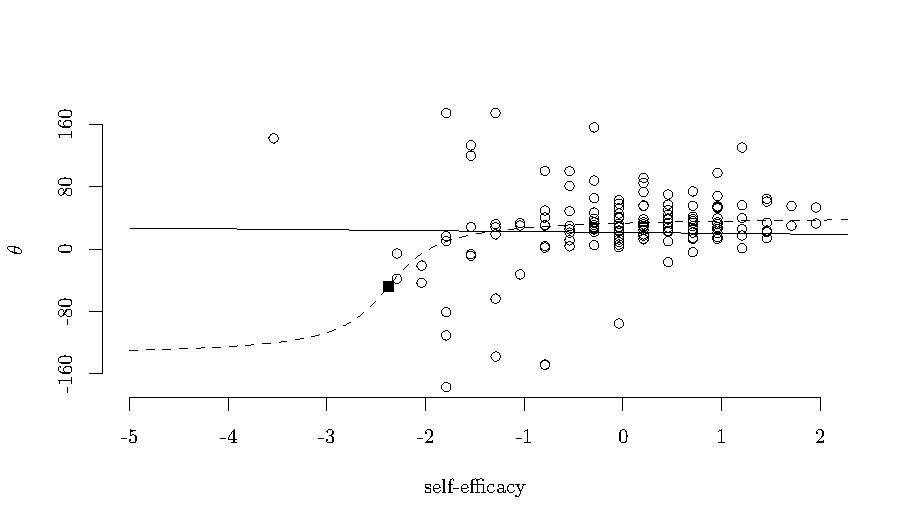
\includegraphics[width = \textwidth]{Plots/reglinediffSE.pdf}
\caption{Plot showing circular regression lines for the effect of self-efficacy
as predicted by the Abe-Ley model (solid line) and CL-PN model (dashed line). The
black square indicates the inflection point of the circular regression line for
the CL-PN model.}
\label{regline}
\end{figure}

\subsubsection{The modified Abe-Ley model} \label{resAL}

\begin{table}

\caption{\label{tab:estAL}Results, cross-validation mean and standard deviation, for the modified Abe-Ley model}
\centering
\begin{tabular}[t]{ll}
\toprule
\multicolumn{1}{c}{Parameter} & \multicolumn{1}{c}{ML-estimate} \\
\cmidrule(l{2pt}r{2pt}){1-1} \cmidrule(l{2pt}r{2pt}){2-2}
$\eta_0$ & 0.36 (0.02)\\
$\eta_1$ & -0.03 (0.01)\\
$\nu_0$ & 1.17 (0.02)\\
$\nu_1$ & 0.04 (0.02)\\
$\alpha$ & 3.66 (0.12)\\
$\kappa$ & 1.51 (0.08)\\
$\lambda$ & 0.70 (0.05)\\
\bottomrule
\end{tabular}
\end{table}

First recall the regression equations predicting the linear outcome
\[\hat{\mu}_{i} = \eta_0 + 2 * \tan^{-1}(\eta_1\text{SE}_i)\]

\noindent and circular outcome
\[\hat{\beta}_{i} = \exp(\nu_0 + \nu_1\text{SE}_i).\]

\noindent Here \(\hat{\mu}\) is the predicted mean vector of the type of
interpersonal behavior and \(\hat{\beta}\) is the predicted scale
parameter of the strength of interpersonal behavior, while the
\(\eta\)'s and \(\nu\)'s are regression parameters.\newline
\indent Table \ref{tab:estAL} shows the results for the modified Abe-Ley
model fit to the teacher dataset. The estimates in this table are the
averages and standard deviations of the 10 cross-validation estimates.
The estimate of the circular mean at an average self-efficacy,
\(\eta_0\), equals 0.36 radians or 20.62\(^\circ\). For the Abe-Ley
model we can also investigate the effect of self-efficacy on the type of
interpersonal behavior. The solid line in Figure \ref{regline} shows
this effect. Unlike for the regression line of the CL-PN model, the
inflection point of the regression line of the Abe-Ley model lies
outside the x-range of the figure. \newline
\indent For the Abe-Ley model the conditional distribution for the
linear outcome is Weibull. This means that we can use methods from
survival analsis to interpret the effect of self-efficacy. In survival
analysis a `survival' function is used in which time is plotted against
the probability of survival of subjects suffering from a specific
medical condition. In our data however we plot the strength on the IPC
against the probability of a teacher having such a strength. This
probability is computed using the `survival-function'
\(\exp(-\alpha y_i^{\beta(1-\tanh(\kappa)\cos(\theta_i - \mu_i))^{1/\alpha}})\)
with \(\beta = \exp(\nu_0 + \nu_1\mbox{SE}_i)\). In Figure
\ref{reglineweib}, we plot the survival function for the minimum, median
and maximum value of self-efficacy. We conclude that stronger
interpersonal behaviors are less probable. We also see that the relation
between self-efficacy and the strength on the IPC is not linear; the
probability of having a stronger interpersonal behavior is higher for
both the minimum and maximum self-efficacy compared to a median
self-efficacy score. Note however that the circular outcome also
influences the survival function. The relation between the type of
interpersonal behavior and the strength of interpersonal behavior may
thus influence the shape of the survival function.\newline

\begin{figure}
\centering
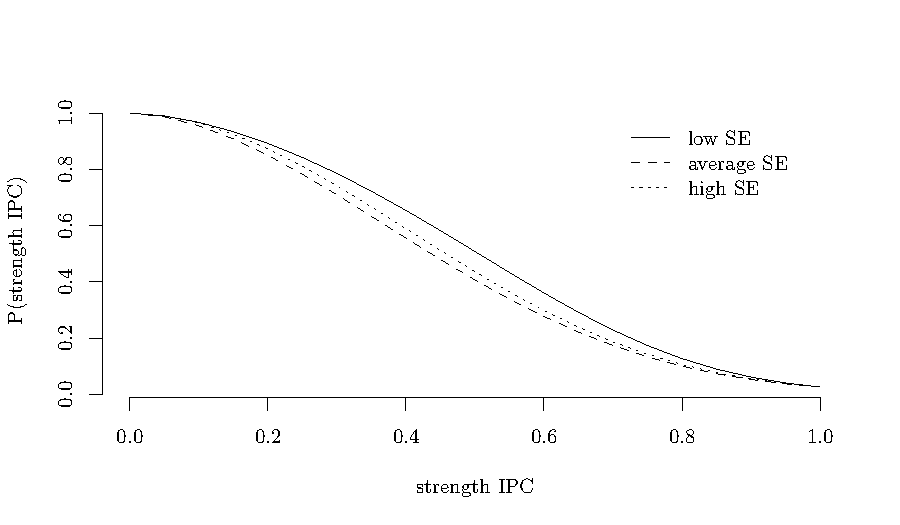
\includegraphics[width = \textwidth]{Plots/survivaldiffSE.pdf}
\caption{Plot showing the probability of having a particular strength of interpersonal behavior (survival plot) for the minimum, mean and maximum self-efficacy in the data.}
\label{reglineweib}
\end{figure}

\subsubsection{The modified GPN-SSN model} \label{resGPNSSN}

\begin{table}
\caption{\label{tab:estCLGPNM}Results, cross-validation mean and standard deviation, for the GPN-SSN model}
\centering
\begin{tabular}[t]{lllllll}
\toprule
\multicolumn{1}{c}{Parameter} & \multicolumn{3}{c}{Unconstrained} & \multicolumn{3}{c}{Constrained} \\
\cmidrule(l{2pt}r{2pt}){1-1} \cmidrule(l{2pt}r{2pt}){2-4} \cmidrule(l{2pt}r{2pt}){5-7}
  & Mode & HPD LB & HPD UB & Mode & HPD LB & HPD UB\\
\midrule
$\beta_{0_s^{I}}$ & 0.30 (0.01) & 0.26 (0.01) & 0.34 (0.01) & 2.11 (0.10) & 1.75 (0.09) & 2.50 (0.11)\\
$\beta_{0_s^{II}}$ & 0.19 (0.00) & 0.17 (0.01) & 0.21 (0.00) & 1.33 (0.07) & 1.10 (0.05) & 1.57 (0.06)\\
$\beta_{0_y}$ & 0.33 (0.01) & 0.30 (0.30) & 0.36 (0.01) & 0.33 (0.01) & 0.30 (0.01) & 0.36 (0.01)\\
$\beta_{1_s^{I}}$ & 0.09 (0.01) & 0.05 (0.01) & 0.13 (0.01) & 0.60 (0.06) & 0.33 (0.05) & 0.90 (0.06)\\
$\beta_{1_s^{II}}$ & 0.07 (0.00) & 0.04 (0.00) & 0.09 (0.01) & 0.48 (0.03) & 0.30 (0.03) & 0.66 (0.04)\\
\addlinespace
$\beta_{1_y}$ & 0.09 (0.01) & 0.06 (0.06) & 0.12 (0.01) & 0.09 (0.01) & 0.06 (0.01) & 0.12 (0.01)\\
$\sum_{s_{1,1}}$ & 0.05 (0.00) & 0.04 (0.00) & 0.06 (0.00) & 2.43 (0.14) & 1.72 (0.07) & 3.46 (0.13)\\
$\sum_{s_{2,2}}$ & 0.02 (0.00) & 0.02 (0.00) & 0.03 (0.00) & 1.00 (0.00) & 1.00 (0.00) & 1.00 (0.00)\\
$\sum_{y_{3,3}}$ & 0.03 (0.00) & 0.02 (0.02) & 0.04 (0.00) & 0.03 (0.00) & 0.02 (0.00) & 0.04 (0.00)\\
$\sum_{s_{1,2}}$ & 0.00 (0.00) & -0.00 (0.00) & 0.01 (0.00) & 0.07 (0.06) & -0.20 (0.06) & 0.35 (0.06)\\
\addlinespace
$\sum_{sy_{1,3}}$ & 0.03 (0.00) & 0.02 (0.00) & 0.04 (0.00) & 0.23 (0.01) & 0.17 (0.01) & 0.32 (0.01)\\
$\sum_{sy_{2,3}}$ & 0.01 (0.00) & 0.01 (0.01) & 0.02 (0.00) & 0.09 (0.01) & 0.06 (0.01) & 0.12 (0.01)\\
$\lambda$ & 0.16 (0.01) & 0.14 (0.01) & 0.18 (0.01) & 0.16 (0.01) & 0.14 (0.01) & 0.18 (0.01)\\
\bottomrule
\end{tabular}
\end{table}

First recall the regression equation predicting the circular and linear
outcome:

\[\hat{\boldsymbol{\mu}}_{i} = \boldsymbol{\beta}_0 +\boldsymbol{\beta}_1\text{SE}_i,\]

\noindent where
\(\boldsymbol{\mu}_i = (\boldsymbol{\mu}_{s_i}, \boldsymbol{\mu}_{y_i})^t\),
\(\boldsymbol{\beta}_0 = (\beta_{0_{s^{I}}}, \beta_{0_{s^{II}}},\beta_{0_y})^t\)
and
\(\boldsymbol{\beta}_1 = (\beta_{1_{s^{I}}}, \beta_{1_{s^{II}}},\beta_{1_y})^t\).
The parameters \(\beta_{0_{s^{I}}}\), \(\beta_{0_{s^{II}}}\),
\(\beta_{1_{s^{I}}}\) and \(\beta_{1_{s^{II}}}\) are the intercepts and
regression coefficients for the circular outcome and \(\beta_{0_y}\) and
\(\beta_{1_y}\) are the intercept and regression coefficient for the
linear outcome.\newline
\indent Table \ref{tab:estCLGPNM} shows the results for the modified
GPN-SSN model fit to the teacher dataset. The estimates in this table
are the averages and standard deviations of the 10 cross-validation
estimates. We show both the estimated posterior mode and the 95\%
highest posterior density (HPD) interval for each parameter. The
predicted circular means can be computed from \(\beta_{0_{s^{I}}}\) and
\(\beta_{0_{s^{II}}}\) in a similar fashion as for the CL-PN and CL-GPN
models. Table \ref{tab:means} shows the posterior mode of the estimated
circular mean, which equals 35.30\(^\circ\) and hence is very similar to
those of the CL-PN and CL-GPN models.\newline
\indent For the same reason as in the CL-GPN model we cannot compute
circular regression coefficients for the effect of self-efficacy on the
type of interpersonal behavior such as the \(b_c\) and \(SAM\). Instead,
we will again compute posterior predictive distributions for the
predicted circular outcome of individuals scoring the minimum, maximum
and median self-efficacy. The modes and 95\% HPD intervals of these
posterior predictive distributions are
\(\hat{\theta}_{SE_{min}} = 206.87^\circ (117.11^\circ, \: 72.02^\circ)\),
\(\hat{\theta}_{SE_{median}} = 24.68^\circ (334.73^\circ, \: 128.27^\circ)\),
\(\hat{\theta}_{SE_{max}} = 29.81^\circ (0.74^\circ, \: 80.61^\circ)\).
On a circle the HPD intervals of the three posterior predictive
distributions overlap. Had they not overlapped we could have concluded
that as the self-efficacy increases, the score of the teacher on the IPC
moves counterclockwise. The effect of self-efficacy on the strength of
interpersonal behavior is quantified by \(\beta_{1_y}\), and we learn
that for a 1 unit increase in self-efficacy the strength of
interpersonal behavior increases by 0.09. The average strength is
quantified by \(\beta_{0_y}\) and equals 0.33.\newline
\indent To investigate the association between the linear and circular
outcome we look at the covariances between the linear outcome and the
sine and cosine of the circular outcome \(\sum_{sy_{2,3}}\) and
\(\sum_{sy_{1,3}}\). Both covariances, \(\sum_{sy_{2,3}} = 0.09\) and
\(\sum_{sy_{1,3}} = 0.23\), are different from zero, but the one of the
cosine component is larger. This means the correlation with the
Communion component is larger and that teachers scoring both high on
Communion and Agency show stronger behavior. This is a slightly
different conclusion from the one in the CL-PN and CL-GPN models.

\subsubsection{Model fit}

In this section we will assess the overall fit of the cylindrical models
to the data via the PLSL criterion described in Section \ref{Modelfit}.
Table \ref{tab:ModelFit} shows the values of this criterion for the
linear and circular outcomes of the four models.\newline
\indent The CL-PN and CL-GPN models have the best out-of-sample
predictive performance for the linear outcome. They show roughly the
same performance because they model the linear outcome in the same way.
Only the value of \(r\) in \eqref{circlinlink} differs. We should note
that even though the predictive performance of the Abe-Ley model for the
linear outcome is worst on average, the standard deviation of the
cross-validation estimates is rather large. This means that in some
samples, the Abe-Ley model shows a lower PLSL value than the average of
25.49\newline
\indent The Abe-Ley model has the best out-of-sample predictive
performance for the circular outcome. This would suggest that for the
circular variable a slightly skewed distribution fits best. However,
both the GPN-SSN and the CL-GPN models fit much worse even though the
distribution for the circular outcome in these models can also take a
skewed shape. It should be noted that the standard deviation of the
cross-validation estimates is rather large for the Abe-Ley and the
CL-GPN model. It is possible that these large standard deviations for
the PLSL are caused by the fact that they are computed for a relatively
small sample size, but this does not explain why the PLSL has a large
standard deviation for only a few cylindrical models and not for all.

\begin{table}

\caption{\label{tab:ModelFit}PLSL criteria, cross-validation mean and standard deviation, for the circular and linear outcome in the four cylindrical models}
\centering
\begin{tabular}[t]{lrlrl}
\toprule
\multicolumn{1}{c}{Model} & \multicolumn{2}{c}{Circular} & \multicolumn{2}{c}{Linear} \\
\cmidrule(l{2pt}r{2pt}){1-1} \cmidrule(l{2pt}r{2pt}){2-3} \cmidrule(l{2pt}r{2pt}){4-5}
  & mean & sd & mean & sd\\
\midrule
CL-PN & 82.96 & (9.47) & -17.65 & (3.70)\\
CL-GPN & 85.22 & (18.12) & -18.12 & (3.57)\\
Abe-Ley & 31.97 & (22.07) & 25.49 & (17.46)\\
GPN-SSN & 106.38 & (8.84) & -2.14 & (6.78)\\
\bottomrule
\end{tabular}
\end{table}

\section{Discussion}\label{Discussion}

In this paper we modified four models for cylindrical data in such a way
that they include a regression of both the linear and circular outcome
onto a set of covariates. Subsequently we have shown how these four
methods can be used to analyze a dataset on the interpersonal behavior
of teachers. In this final section we will comment on the differences
between these models, the results from the analysis of the teacher data
and how cylindrical models improve the analysis of such cylindrical
data.\newline
\indent In terms of interpretability, the CL-PN and Abe-Ley models
perform best. In the CL-GPN and GPN-SSN models the interpretation of the
parameters of the circular outcome component is not straightforward, if
at all possible. This is caused by the fact that in addition to the mean
vector the covariance matrix of the GPN distribution affects the
location of the circular data, making it difficult to compute regression
coefficients on the circle. Wang \& Gelfand (2013) state that Monte
Carlo integration can be used to compute a circular mean and variance
for the GPN distribution. In future research, this solution might be
applied to the methods of Cremers et al. (2018b) in order to compute
circular coefficients for GPN models.\newline
\indent In terms of flexibility the GPN-SSN model scores best. Multiple
linear and circular outcomes can be included and we can thus apply the
model to multivariate cylindrical data. In addition the GPN-SSN, the
CL-GPN and CL-PN models are extendable to a mixed-effects structure and
can thus also be fit to longitudinal data (see Nuñez-Antonio \&
Gutiérrez-Peña (2014) and Hernandez-Stumpfhauser et al. (2016) for
hierarchical/mixed-effects models for the PN and GPN distributions
respectively). For the Abe-Ley model this may also be possible but has
not been done in previous research for the conditional distribution of
its circular outcome (sine-skewed von Mises). Concerning asymmetry, both
the GPN-SSN as well as the Abe-Ley model allow for non-symmetrical
shapes of the distributions of both the linear and circular outcome,
while the CL-GPN model permits an asymmetric circular outcome.\newline
\indent To investigate model fit for the teacher data, we assessed
out-of-sample predictive performance for both the linear and circular
outcome. The CL-PN and CL-GPN models have the best fit for the linear
outcome while the Abe-Ley model fits best the circular outcome.
Differences in fit, in addition to being a result of different
distributional assumptions, may also be caused by the way in which the
relation between the linear and circular outcome is modeled. Whereas in
both the Abe-Ley and GPN-SSN models the distribution of the linear
outcome is conditioned on the circular outcome and vice versa, the
distribution of the circular outcome in the CL-PN and CL-GPN models is
independent of the linear outcome. In these models the circular outcome
is regressed onto the linear outcome.\newline
\indent The four cylindrical models that were modified to the regression
context in this paper are not the only cylindrical distributions
available from the literature. Other interesting cylindrical
distributions have been introduced by Fernández-Durán (2007), Kato \&
Shimizu (2008) and Sugasawa (2015) (for more references we refer to
Chapter 2 of Ley \& Verdebout (2017)). In the present study we have
decided not to include these distributions for reasons of space,
complexity of the models and ease of implementing a regression
structure. In future research however it would be interesting to
investigate other types of cylindrical distributions as well in order to
compare the interpretability, flexibility and model fit to the models
developed in the present study.\newline
\indent We conclude the paper on a general note regarding cylindrical
models. They offer new insights into data of a cylindrical nature in
psychology. Concerning the example used in this paper, the advantage of
cylindrical data analysis is that we were able to analyze all circular
and linear information in the data simultaneously. In previous research,
the two components of the interpersonal circumplex (\emph{i.e.}, Agency
and Communion) were analyzed separately. Such an approach also provides
information about the strength of teachers' score on Agency and
Communion, yet a large portion of information about the combination of
Agency and Communion, which describes the kind of behavior that is
observed, gets lost. A first solution to include both dimensions as a
circular variable in data analysis was described by Cremers et al.
(2018a). A downside of that analysis was that information about the
strength of the specific type of interpersonal behavior could not be
retained. In the present study, we have shown how using cylindrical
models can simultaneously model the information about the type of and
strength of interpersonal behavior and how these are influenced by
teachers' self-efficacy in classroom management. The results of the
present study therefore provide an answer to an often stated problem in
data analysis of interpersonal circumplex data.

\section*{References}
\DeclareRobustCommand{\VANDER}[3]{#3}


\hypertarget{ref-abe2017tractable}{}
Abe, T., \& Ley, C. (2017). A tractable, parsimonious and flexible model
for cylindrical data, with applications. \emph{Econometrics and
Statistics}, \emph{4}, 91--104.
doi:\href{https://doi.org/10.1016/j.ecosta.2016.04.001}{10.1016/j.ecosta.2016.04.001}

\hypertarget{ref-chrastil2017rotational}{}
Chrastil, E. R., \& Warren, W. H. (2017). Rotational error in path
integration: Encoding and execution errors in angle reproduction.
\emph{Experimental Brain Research}, \emph{235}(6), 1885--1897.
doi:\href{https://doi.org/10.1007/s00221-017-4910-y}{10.1007/s00221-017-4910-y}

\hypertarget{ref-Claessens2016side}{}
Claessens, L. C. (2016). \emph{Be on my side i'll be on your side :
Teachers' perceptions of teacher--student relationships} (PhD thesis).

\hypertarget{ref-Cremers2018Assessing}{}
Cremers, J., Mainhard, M. T., \& Klugkist, I. (2018a). Assessing a
Bayesian embedding approach to circular regression models.
\emph{Methodology}, \emph{14}(2), 69--81.

\hypertarget{ref-CremersMulderKlugkist2017}{}
Cremers, J., Mulder, K. T., \& Klugkist, I. (2018b). Circular
interpretation of regression coefficients. \emph{British Journal of
Mathematical and Statistical Psychology}, \emph{71}(1), 75--95.
doi:\href{https://doi.org/10.1111/bmsp.12108}{10.1111/bmsp.12108}

\hypertarget{ref-fernandez2007models}{}
Fernández-Durán, J. (2007). Models for circular--linear and
circular--circular data constructed from circular distributions based on
nonnegative trigonometric sums. \emph{Biometrics}, \emph{63}(2),
579--585.
doi:\href{https://doi.org/10.1111/j.1541-0420.2006.00716.x}{10.1111/j.1541-0420.2006.00716.x}

\hypertarget{ref-fisher1995statistical}{}
Fisher, N. I. (1995). \emph{Statistical analysis of circular data}.
Cambridge: Cambridge University Press.

\hypertarget{ref-garcia2014test}{}
García-Portugués, E., Barros, A. M., Crujeiras, R. M.,
González-Manteiga, W., \& Pereira, J. (2014). A test for
directional-linear independence, with applications to wildfire
orientation and size. \emph{Stochastic Environmental Research and Risk
Assessment}, \emph{28}(5), 1261--1275.
doi:\href{https://doi.org/10.1007/s00477-013-0819-6}{10.1007/s00477-013-0819-6}

\hypertarget{ref-garcia2013exploring}{}
García-Portugués, E., Crujeiras, R. M., \& González-Manteiga, W. (2013).
Exploring wind direction and SO2 concentration by circular--linear
density estimation. \emph{Stochastic Environmental Research and Risk
Assessment}, \emph{27}(5), 1055--1067.
doi:\href{https://doi.org/10.1007/s00477-012-0642-5}{10.1007/s00477-012-0642-5}

\hypertarget{ref-BDA}{}
Gelman, A., Carlin, J., Stern, H., Dunson, D., Vehtari, A., \& Rubin, D.
(2014). \emph{Bayesian data analysis} (3rd ed.). Boca Raton, FL: Chapman
\& Hall/CRC.

\hypertarget{ref-gneiting2007strictly}{}
Gneiting, T., \& Raftery, A. E. (2007). Strictly proper scoring rules,
prediction, and estimation. \emph{Journal of the American Statistical
Association}, \emph{102}(477), 359--378.
doi:\href{https://doi.org/10.1198/016214506000001437}{10.1198/016214506000001437}

\hypertarget{ref-gurtman2009exploring}{}
Gurtman, M. B. (2009). Exploring personality with the interpersonal
circumplex. \emph{Social and Personality Psychology Compass},
\emph{3}(4), 601--619.
doi:\href{https://doi.org/10.1111/j.1751-9004.2009.00172.x}{10.1111/j.1751-9004.2009.00172.x}

\hypertarget{ref-hernandez2016general}{}
Hernandez-Stumpfhauser, D., Breidt, F. J., \& Woerd, M. J. van der.
(2016). The general projected normal distribution of arbitrary
dimension: Modeling and Bayesian inference. \emph{Bayesian Analysis},
\emph{12}(1), 113--133.
doi:\href{https://doi.org/10.1214/15-BA989}{10.1214/15-BA989}

\hypertarget{ref-horowitz2010handbook}{}
Horowitz, L. M., \& Strack, S. (2011). \emph{Handbook of interpersonal
psychology: Theory, research, assessment, and therapeutic
interventions}. Hoboken, NJ: John Wiley \& Sons.

\hypertarget{ref-jammalamadaka2001topics}{}
Jammalamadaka, S. R., \& Sengupta, A. (2001). \emph{Topics in circular
statistics} (Vol. 5). World Scientific.

\hypertarget{ref-johnson1978some}{}
Johnson, R. A., \& Wehrly, T. E. (1978). Some angular-linear
distributions and related regression models. \emph{Journal of the
American Statistical Association}, \emph{73}(363), 602--606.

\hypertarget{ref-kato2008dependent}{}
Kato, S., \& Shimizu, K. (2008). Dependent models for observations which
include angular ones. \emph{Journal of Statistical Planning and
Inference}, \emph{138}(11), 3538--3549.
doi:\href{https://doi.org/10.1016/j.jspi.2006.12.009}{10.1016/j.jspi.2006.12.009}

\hypertarget{ref-lagona2015hidden}{}
Lagona, F., Picone, M., Maruotti, A., \& Cosoli, S. (2015). A hidden
Markov approach to the analysis of space--time environmental data with
linear and circular components. \emph{Stochastic Environmental Research
and Risk Assessment}, \emph{29}(2), 397--409.
doi:\href{https://doi.org/10.1007/s00477-014-0919-y}{10.1007/s00477-014-0919-y}

\hypertarget{ref-ley2017modern}{}
Ley, C., \& Verdebout, T. (2017). \emph{Modern directional statistics}.
Chapman \& Hall/CRC Press. Boca Raton, FL.

\hypertarget{ref-mardia2000directional}{}
Mardia, K. V., \& Jupp, P. E. (2000). \emph{Directional statistics}
(Vol. 494). Chichester, England: Wiley.

\hypertarget{ref-mardia1978model}{}
Mardia, K. V., \& Sutton, T. W. (1978). A model for cylindrical
variables with applications. \emph{Journal of the Royal Statistical
Society Series B (Methodological)}, \emph{40}(2), 229--233.

\hypertarget{ref-mastrantonio2018joint}{}
Mastrantonio, G. (2018). The joint projected normal and skew-normal: A
distribution for poly-cylindrical data. \emph{Journal of Multivariate
Analysis}, \emph{165}, 14--26.
doi:\href{https://doi.org/10.1016/j.jmva.2017.11.006}{10.1016/j.jmva.2017.11.006}

\hypertarget{ref-mastrantonio2015bayesian}{}
Mastrantonio, G., Maruotti, A., \& Jona-Lasinio, G. (2015). Bayesian
hidden Markov modelling using circular-linear general projected normal
distribution. \emph{Environmetrics}, \emph{26}(2), 145--158.
doi:\href{https://doi.org/10.1002/env.2326}{10.1002/env.2326}

\hypertarget{ref-nunez2014bayesian}{}
Nuñez-Antonio, G., \& Gutiérrez-Peña, E. (2014). A Bayesian model for
longitudinal circular data based on the projected normal distribution.
\emph{Computational Statistics \& Data Analysis}, \emph{71}, 506--519.
doi:\href{https://doi.org/10.1016/j.csda.2012.07.025}{10.1016/j.csda.2012.07.025}

\hypertarget{ref-nunez2011bayesian}{}
Nuñez-Antonio, G., Gutiérrez-Peña, E., \& Escarela, G. (2011). A
Bayesian regression model for circular data based on the projected
normal distribution. \emph{Statistical Modelling}, \emph{11}(3),
185--201.
doi:\href{https://doi.org/10.1177/1471082X1001100301}{10.1177/1471082X1001100301}

\hypertarget{ref-olmos2012extension}{}
Olmos, N. M., Varela, H., Gómez, H. W., \& Bolfarine, H. (2012). An
extension of the half-normal distribution. \emph{Statistical Papers},
\emph{53}(4), 875--886.
doi:\href{https://doi.org/10.1007/s00362-011-0391-4}{10.1007/s00362-011-0391-4}

\hypertarget{ref-pennings2018interpersonal}{}
Pennings, H. J. M., Brekelmans, M., Sadler, P., Claessens, L. C.,
\VANDER{Want}{Van der}{van der} Want, A. C., \& Tartwijk, J. van.
(2018). Interpersonal adaptation in teacher-student interaction.
\emph{Learning and Instruction}, \emph{55}, 41--57.
doi:\href{https://doi.org/10.1016/j.learninstruc.2017.09.005}{10.1016/j.learninstruc.2017.09.005}

\hypertarget{ref-rayner200935th}{}
Rayner, K. (2009). The 35th Sir Frederick Bartlett lecture: Eye
movements and attention in reading, scene perception, and visual search.
\emph{Quarterly Journal of Experimental Psychology}, \emph{62}(8),
1457--1506.
doi:\href{https://doi.org/10.1080/17470210902816461}{10.1080/17470210902816461}

\hypertarget{ref-sahu2003new}{}
Sahu, S. K., Dey, D. K., \& Branco, M. D. (2003). A new class of
multivariate skew distributions with applications to Bayesian regression
models. \emph{Canadian Journal of Statistics}, \emph{31}(2), 129--150.
doi:\href{https://doi.org/10.2307/3316064}{10.2307/3316064}

\hypertarget{ref-sugasawa2015flexible}{}
Sugasawa, S., S. (2015). \emph{A flexible family of distributions on the
cylinder}. Retrieved from
\href{arXiv:\%201501.06332v2}{arXiv: 1501.06332v2}

\hypertarget{ref-wang2012directional}{}
Wang, F., \& Gelfand, A. E. (2013). Directional data analysis under the
general projected normal distribution. \emph{Statistical Methodology},
\emph{10}(1), 113--127.
doi:\href{https://doi.org/10.1016/j.stamet.2012.07.005}{10.1016/j.stamet.2012.07.005}

\hypertarget{refs}{}
\hypertarget{ref-vanderWant2015role}{}
\VANDER{Want}{Van der}{van der} Want, A. C. (2015). \emph{Teachers'
interpersonal role identity.} (PhD thesis).

\hypertarget{ref-wubbels2006interpersonal}{}
Wubbels, T., Brekelmans, M., Brok, P. den, \& Tartwijk, J. van. (2006).
An interpersonal perspective on classroom management in secondary
classrooms in the Netherlands. In C. Evertson \& C. S. Weinstein (Eds.),
\emph{Handbook of classroom management: Research, practice, and
contemporary issues} (pp. 1161--1191). Malwah, NJ: Lawrence Erlbaum
Associates.


\end{document}
